
\chapter{Objetivos}
\label{cap:Objetivo}

Tal y como se ha mencionado previamente, el consumo de energía en sistemas informáticos es un tema de extremada relevancia, en la actualidad, muy tenido en cuenta en todas las etapas de desarrollo de los mismos. Esto es debido a que, en los últimos años, las prestaciones de los \ac{SoC} han aumentado exponencialmente, posibilitando aspectos que, hasta ahora, eran únicamente posibles de lograr con un ordenador de sobremesa. Esto ha llevado consigo un aumento constante en el consumo energético de estos \textit{chips}. Según \cite{energiaSoc}, con una gráfica del \ac{ITRS} del año 2011, el consumo medio de los \ac{SoC} destinados a dispositivos portátiles se ha incrementado desde el año 2010 hasta la actualidad en un 405\%. Si bien para este año 2024, las previsiones no se han cumplido, los valores reales son cercanos con el lanzamiento del \ac{SoC} tope de gama de Qualcomm, el Snapdragon 8 Gen 3, presentando un \ac{TDP} de 6.3 Vatios \cite{snapdragon8}, y además reducido por el propio fabricante, siendo del 315\%. 

\begin{figure}[H]
    \centering
    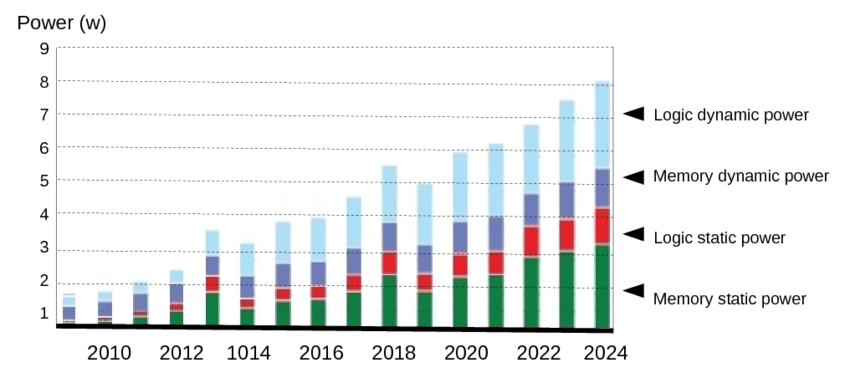
\includegraphics[width=0.95\linewidth, height=0.45\textwidth]{figs/itrs-previsiones.png}
    \caption{Estimaciones sobre la potencia requerida en semiconductores, año 2011 ~\cite{energiaSoc}.}
\end{figure}

Esta problemática creciente ha motivado a los principales diseñadores y fabricantes de semiconductores a profundizar en técnicas de estimación y validación de energía consumida en las arquitecturas desarrolladas. Dentro de este contexto, es interesante, por tanto, la realización de estimaciones para comprobar la energía consumida ante diferentes cargas de trabajo en este tipo de sistemas, obteniéndose una cota superior y así validar energéticamente la plataforma de cómputo en cuestión.

Una técnica de estimación de consumo de energía son los entornos de simulación \textit{hardware}, aquellos especializados en replicar una arquitectura real de forma precisa, proporcionando una validación a nivel de ciclo, y no meramente funcional. Este factor hace que sea viable la estimación del consumo de energía de una arquitectura real mediante la ejecución de simulaciones basadas en la misma. El objetivo principal es, por tanto, el desarrollo y evaluación un modelo de consumo energético para aplicaciones intensivas en cómputo en procesadores \ac{ARM}, utilizando análisis de estadísticas de ejecución de bajo nivel (contadores hardware), con el fin de estimar con precisión el consumo de energía y proporcionar una base técnica para predecir el tiempo de vida útil de los sistemas. 

Para alcanzar este objetivo, se realizará un marco de medición que establezca un modelo de consumo, enfocado en los componentes más relevantes dentro de la plataforma, así como de su peso dentro de la misma. Este modelo se trasladará al simulador, para la obtención de métricas de consumo gracias a la obtención de las estadísticas necesarias, fruto de la ejecución de las diferentes simulaciones. Más adelante, los resultados obtenidos en el simulador se validarán, ejecutándose sobre la plataforma real exactamente lo mismo que se ejecutó sobre la arquitectura simulada, verificándose la correctitud del modelo.

El objetivo principal mencionado anteriormente se basa, a su vez, en una serie de objetivos parciales o secundarios:

\begin{enumerate}
    \item Definición de un modelo de sistema basado en arquitecturas \ac{ARM}, así como la de un modelo teórico de energía y una selección de \textit{benchmarks} intensivos en cómputo para su posterior validación. 

    \item Análisis y experimentación de herramientas que permitan la obtención de métricas de ejecución a bajo nivel, que permitan la monitorización en tiempo real sobre un conjunto de \textit{benchmarks} intensivos en cómputo ejecutados en procesadores \ac{ARM} y una mínima interferencia de factores externos, como la captura de valores de contadores \textit{hardware} o el despliegue de simulaciones del modelo de sistema, externos, con el propósito de obtener el consumo energético del sistema.
    
    %\item Modelar con el simulador gem5 la arquitectura de cómputo de los procesadores \ac{ARM}, específicamente la arquitectura de una Raspberry Pi 4, para proporcionar datos de consumo energético de un conjunto de \textit{benchmarks}, de manera que se puedan comparar con los resultados obtenidos a través de los contadores de hardware.iseño del conjunto de  experimentos e instrumentación necesaria para la medición del consumo energético real de aplicaciones en al menos dos plataformas de cómputo Raspberry Pi. 

    \item Deducción, a partir de los resultados obtenidos, un modelo de consumo energético, que permita la caracterización fiable y precisa del consumo energético de aplicaciones intensivas en cómputo que ejecutan sobre la arquitectura \ac{ARM}.

    \item Comparación del modelo desarrollado con otros modelos de energía estudiados, en términos de precisión y fiabilidad y proporcionar un análisis de las ventajas y limitaciones del modelo desarrollado en comparación con los modelos existentes. \\
\end{enumerate}

En los siguientes capítulos de este \ac{TFM} se irán mostrando los pasos realizados para el cumplimiento de estos objetivos, y así dar por cumplido también el objetivo principal del trabajo.
